\documentclass{article}
\usepackage[utf8]{inputenc}
\usepackage{graphicx}
\usepackage[utf8]{inputenc}
\usepackage{amssymb}
\usepackage{caption}
\usepackage{subcaption}
\usepackage{array}
\usepackage{tabularx}


\title{\textbf{\Huge Movie Recommendation System using K-Means}}
\author{\Large Kranti Kumari: 202SP011, Nikhil Bobate - 202SP017 \\ Under the guidance of Dr. Aparna P\\\\ Department of Electronics and Communication Engineering\\ National Institute of Technology, Surathkal\\  Karnataka-575025, India}
\date{May 2021}

\begin{document}

\maketitle

\begin{flushleft}
\textbf{\large 1. Abstract}
\end{flushleft}

Recommender system is a filtration program whose prime goal is to predict the “rating” or “preference” of a user towards a domain-specific item or item. In our case, this domain-specific item is a movie, therefore the main focus of our recommendation system is to filter and predict only those movies which a user would prefer, given some data about the user himself or herself. This project aims at implementing a Movie Recommendation system using Memory based, item-to-item Collaborative Approach of K-Means algorithm to reduce the human effort by suggesting movies based on the user’s interests. \\


\begin{flushleft}
\textbf{\large 2. Introduction}
\end{flushleft}

During the last few decades, with the rise of YouTube, Amazon, Netflix and many other such web services, recommender systems have taken more and more place in our lives. They are so commonplace now that many of us use them without even knowing it. Because we can't possibly look through all the products or content on a website, a recommendation system plays an important role in helping us have a better user experience, while also exposing us to more inventory we might not discover otherwise. \\

Different filtration strategies are Content based filtering and Collaborative filtering. \\
In Content Based filtering, the filtration strategy is based on the data provided about the items. The algorithm recommends products that are similar to the ones that a user has liked in the past. This similarity (generally cosine similarity) is computed from the data we have about the items as well as the user’s past preferences.\\
In Collaborative filtering, the filtration strategy is based on the combination of the user’s behavior and comparing and contrasting that with other users’ behavior in the database. The history of all users plays an important role in this algorithm. \\ 
It has two variations: memory based and model based approaches. Memory based approaches directly works with values of recorded interactions, assuming no model, and are essentially based on nearest neighbours search (for example, find the closest users from a user of interest and suggest the most popular items among these neighbours). Model based approaches assume an underlying “generative” model that explains the user-item interactions and try to discover it in order to make new predictions. \\

Figure 1 depicts the Illustration of Content based filtering and Collaborative filtering:

\begin{figure}[htp]
    \centering
    \Large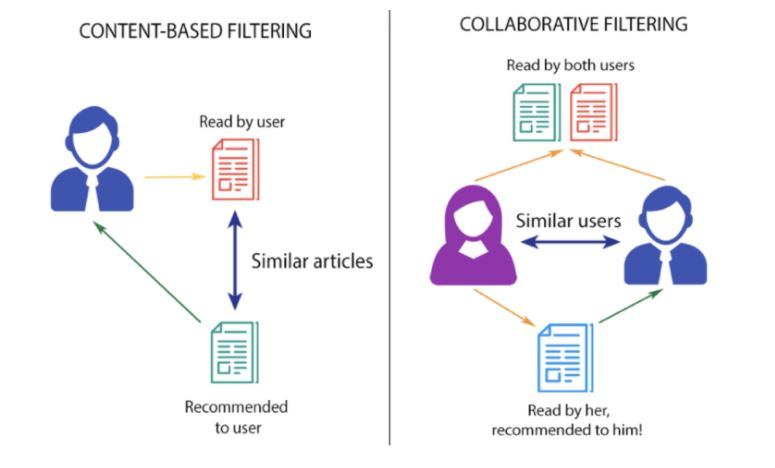
\includegraphics[width=11cm, height=7cm]{FitrationStrategy.JPG}
    \caption{Filtration Strategies}
    \label{fig:FitrationStrategy}
\end{figure}

For this model, we are using Movie Lens Small Latest Data-set from Kaggle.
\\

\begin{flushleft}
\textbf{\large 3. Recommendation System}
\end{flushleft}

Our aim is to reduce the human effort by suggesting movies based on the user’s interests.\\

\begin{flushleft}
\textbf{3.1. Problem Statement}
\end{flushleft}

Content-based recommendation systems are constrained to people, these systems don't prescribe things out of the box. These systems work on individual users’ ratings, hence limiting your choice to explore more. While our system which is based on a collaborative approach computes the connection between different clients and relying upon their ratings, prescribes movies to others who have similar tastes, subsequently allowing users to explore more. It will give progressively explicit outcomes contrasted with different systems that are based on the content-based approach. \\

\begin{flushleft}
\textbf{3.2. Methodology}
\end{flushleft}

Collaborative filtering works based on users that have similar tastes. 

\begin{flushleft}
Figure 2 depicts the Flowchart of our recommendation system:
\end{flushleft}

\begin{figure}[htp]
    \centering
    \Large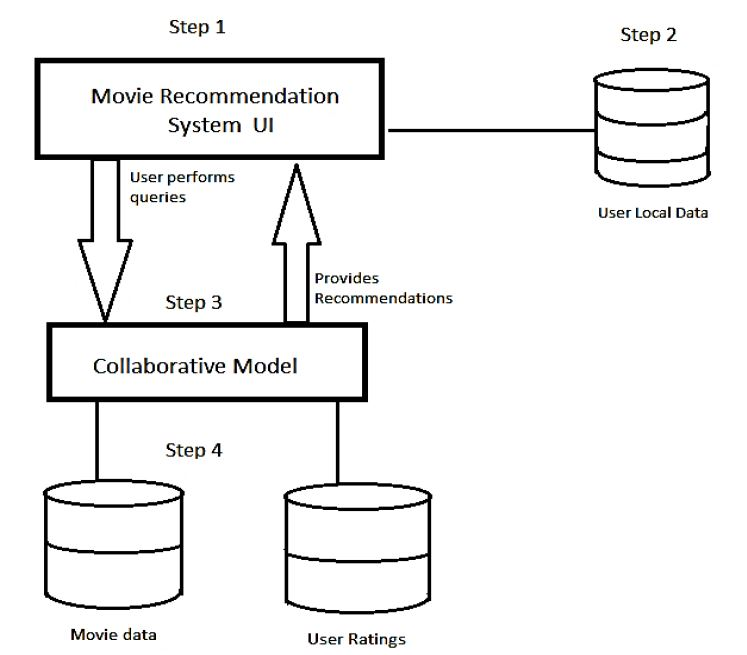
\includegraphics[width=11cm, height=8cm]{Flowchart.JPG}
    \caption{Architecture of movie recommendation system}
    \label{fig:Flowchart}
\end{figure}


\begin{flushleft}
Steps involved in building this model are:
\end{flushleft}


\begin{enumerate}

    \item Cleaning the dataset
        \begin{itemize}
          \item Remove dashes from dataset and identify unique movies that have been rated. 
          \item Remove users who haven’t at least rated 55 movies.
        \end{itemize}
    
    \item Merge datasets
        \begin{itemize}
          \item Combine the two datasets genres and tags for metadata.  
        \end{itemize}
        
    \item Perform dimension reduction
        \begin{itemize}
          \item This dataset gives what we call a sparse matrix. So, perform singular value decomposition (SVD) for dimension reduction which will identify variables that have the most variance.  
        \end{itemize}
        
    \item Run the algorithm for the target film
        \begin{itemize}
          \item Run the collaborative filtering algorithm
        \end{itemize}
        
\end{enumerate}

\begin{center}
\end{center}

\begin{flushleft}
\textbf{\large 4. Results}
\end{flushleft}

The main focus of our recommendation system is to filter and predict only those movies, which a user would prefer, given some data about the user himself or herself.

\begin{flushleft}
Figure 3 depicts the variance plot to see what latent dimensions to use:
\end{flushleft}

\begin{figure}[htp]
    \centering
    \Large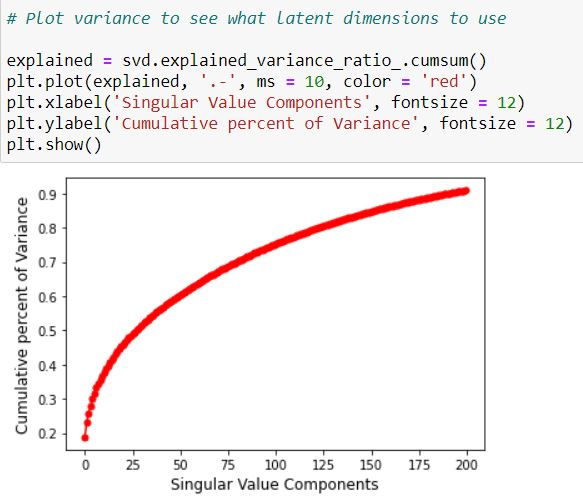
\includegraphics[width=11cm, height=8cm]{VariancePlot.JPG}
    \caption{Variance plot}
    \label{fig:VariancePlot}
\end{figure}

\begin{flushleft}
We then run the collaborative model for the target film. Figure 4 shows the output of our recommendation model for the selected movie 'Toy Story (1995)'.
\end{flushleft}

\begin{figure}[htp]
    \centering
    \Large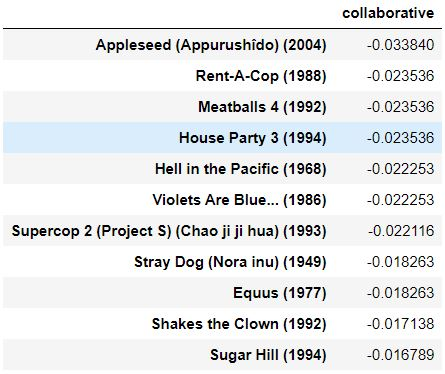
\includegraphics[width=11cm, height=7cm]{Recommend.JPG}
    \caption{Recommendation for Toy Story (1995)}
    \label{fig:Recommend}
\end{figure}


\begin{flushleft}
\textbf{\large 5. Conclusion}
\end{flushleft}

This recommendation system recommends different movies to users. Since this system is based on a collaborative approach, it will give progressively explicit outcomes contrasted with different systems that are based on the content-based approach. Content-based recommendation systems are constrained to people, these systems don't prescribe things out of the box. These systems work on individual users’ ratings, hence limiting your choice to explore more. While our system which is based on a collaborative approach computes the connection between different clients and relying upon their ratings, prescribes movies to others who have similar tastes, subsequently allowing users to explore more.\\


\begin{flushleft}
\textbf{\large 6. References}
\end{flushleft}

[1] F. Furtado, A, Singh, A "Movie Recommendation System Using Machine Learning" : 2020, International Journal of Research in Industrial Engineering, Vol. 9, No. 1 (2020) 84–98  \\

[2] https://towardsdatascience.com/introduction-to-recommender-systems-6c66cf15ada.\\

[3] Duda, Richard O., Peter E. Hart and David G. Stork., “Pattern Classification”, John Wiley and Sons, 2012.\\


\end{document}
